\section{CGSquared \& BiCGStab}
Idee:
\begin{enumerate}
\item Gl\"atte Konvergenz in BiCG !
\item Ersetze Multiplikation mit $A^H$ durch eine mit $A$ und erreiche
 $x^k \in x^0 + K_{2k}(A,r^0)$
\end{enumerate}
Daf�r ben\"otigen wir die folgenden BiCG-Verfahrenspolynome:

\begin{defn}
$\varphi_m \in \overline{\Pi}_m,\ \psi_m \in \Pi_m$ sind die Polynome des BiCG-Verfahrens, d.h.
\[
\varphi_m(A)r^0=r^m,\ \psi_m(A)r^0=p^m.
\]
Dann gilt auch
\[
\overline{\varphi}_m(A^H)\tilde{r}^0=\tilde{r}^m,\ \overline{\psi}_m(A^H)\tilde{r}^0=\tilde{p}^m,
\]
wobei $\varphi_m(t)= \sum_{i=0}^m \beta_i t^i$ und $\overline{\varphi}_m(t)= \sum_{i=0}^m \overline{\beta}_i t^i$.
\end{defn}

\begin{defn}
Auf $\Pi$ = Menge der Polynome ist die Bilinearform $\left[ \cdot , \cdot \right]$ erkl\"art durch:
\[
\left[p,q \right] = \langle p(A)r^0, \overline{q}(A^H)\tilde{r}^0 \rangle.
\]
\end{defn}

\begin{lem}
$\left[ \cdot , \cdot \right]$ ist bilinear und es gilt
\[
\left[p,q \right] = \left[ pq,1 \right]
\]
\[
\left[p \vartheta,q \right] = \left[ p,\vartheta q \right],\ \text{wobei } \vartheta(t)=t.
\]
\end{lem}
Der Beweis ist trivial.
\medskip


Anwendung auf BiCG Koeffizienten:
\[
\langle r^k, \tilde{r}^k \rangle = \left[ \varphi_k, \varphi_k \right] = \left[ \varphi_k^2,1 \right]
\]
\[
\langle Ap^k, \tilde{p}^k \rangle = \left[ \vartheta \psi_k, \psi_k \right] = \left[ \vartheta \psi_k^2,1 \right].
\]
Setze also
\[
\Phi_k = \varphi_k^2 \in \overline{\Pi}_{2k},\ \Psi_k = \psi_k^2 \in \Pi_{2k}.
\]
Wegen
\[r^{k+1} = r^{k} - \gamma_kAp^k \quad\text{und}\quad p^{k+1} = r^{k+1} + \rho_kp^k\]
gilt dann
\[
\Phi_{k+1} = \varphi_{k+1}^2 = \left( \varphi_k - \gamma_k \vartheta \psi_k \right)^2 = \Phi_k -2 \gamma_k \vartheta \varphi_k \psi_k + \gamma_k^2 \vartheta^2 \Psi_k
\]
sowie
\[
\Psi_{k+1} = \psi_{k+1}^2 = \left( \varphi_{k+1} + \rho_k \psi_k \right)^2 = \Phi_{k+1} + 2 \rho_k \varphi_{k+1} \psi_k + \rho_k^2 \Psi_k.
\]
Ohne die gemischten Terme $\varphi_k\psi_k$ in der Gleichung f"ur $\Phi_{k+1}$ und $\phi_{k+1}\psi_k$ in der Gleichung f"ur $\Psi_{k+1}$ h\"atten wir Iterationsvorschriften in $\Phi_k,~\Phi_{k+1}$ und $\Psi_k$. Um diese Iterationsvorschriften zu erhalten, f\"uhren wir einen der gemischten Terme als dritte Gr\"o"se ein. Setzen wir also $\Upsilon_k := \varphi_k\psi_k$, so gilt
\[
\varphi_{k+1} \psi_k = \Upsilon_k - \gamma_k \vartheta \Psi_k
\]
und somit
\[
\Upsilon_{k+1}=\varphi_{k+1} \psi_{k+1} = \Phi_{k+1} + \rho_k \left(\Upsilon_k - \gamma_k \vartheta \Psi_k \right).
\]

Zusammenfassung:
\begin{enumerate}
\item $\gamma_k = \dfrac{\left[\Phi_k,1\right]}{\left[ \vartheta \Psi_k,1 \right]}$
\item $\Phi_{k+1} = \Phi_k - \vartheta \left( 2 \gamma_k \Upsilon_k + \gamma_k^2 \vartheta \Psi_k \right)$
\item $\rho_k = \dfrac{\left[\Phi_{k+1},1 \right]}{\left[ \Phi_k,1 \right] }$
\item $\Upsilon_{k+1} = \Phi_{k+1} + \rho_k \left( \Upsilon_k + \gamma_k \vartheta \Psi_k \right) $
\item $\Psi_{k+1} = \Phi_{k+1} + 2 \rho_k \left( \Upsilon_k - \gamma_k \vartheta \Psi_k \right) + \rho^2_k \Psi_k$
\end{enumerate}

Unter Verwendung der Vektoren $r^k = \Phi_k(A)r^0$, $p^k = \Psi_k(A)r^0$,
$u^k = \Upsilon_k(A)r^0$ und der Iterierten $x^k$ mit $r^k = b-Ax^k$ ergibt
dies folgendes neues Verfahren:
\begin{alg}[CGS (CG-squared, Sommerfeld 1989)]
~               % um "Algorithmus" aus dem Kasten rauszubekommen
\vspace*{-2\baselineskip}       % um den Leeraum zu entfernen
\begin{algorithm}
  \begin{algorithmic} 
    \STATE w\"ahle $x^0$, setze $r^0 = b-Ax^0$, w\"ahle $\tilde{r}^0,\ p^0=r^0=u^0$
    \FOR{$k = 0,1, \dots$ }
	\STATE $s^k=Ap^k$
      \STATE $\gamma_k = \dfrac{\langle r^k, \tilde{r}^0 \rangle}{\langle s^k, \tilde{r}^0 \rangle}$
	\STATE $r^{k+1} = r^k - A\left(2 \gamma_k u^k + \gamma_k^2 s^k \right)$
	\STATE $x^{k+1} = x^k + 2 \gamma_k u^k + \gamma_k^2 s^k$
	\STATE $\rho_k= \dfrac{\langle r^{k+1},\tilde{r}^0 \rangle}{\langle r^k, \tilde{r}^0 \rangle}$
	\STATE $u^{k+1} = r^{k+1} + \rho_k \left( u^k + \gamma_k s^k \right)$
	\STATE $p^{k+1}=r^{k+1} + 2 \rho_k \left( u^k - \gamma_k s^k \right) + \rho^2_k p^k$
    \ENDFOR
  \end{algorithmic}
\end{algorithm}
\end{alg}

\begin{bem}
\begin{enumerate}
\item $x^k \in x^0 + K_{2k}(A,r^0)$ und 2 MVM mit $A$ pro Schritt.
\item $r^k = \varphi_k^2(A)r^0=\varphi_k(A) \underbrace{\varphi_k(A)r^0}_{r_k^\text{BiCG}}$
\end{enumerate}
Ist das wirklich eine Verbesserung? Ein gutes $\varphi_k$ f\"ur $r^0$ ist nicht notwendig ein gutes Polynom f\"ur $\varphi_k(A)r^0$.
Ein schlechtes Polynom $\varphi_k$ f\"ur $r^0$ ist wahrscheinlich auch schlecht f\"ur $\varphi_k(A)r^0$.
Folge: CGS schwankt noch extremer als BiCG.
\end{bem}

\begin{aufg}
F\"uhre CGS f\"ur das Modellproblem III durch.
\end{aufg}

\begin{figure}
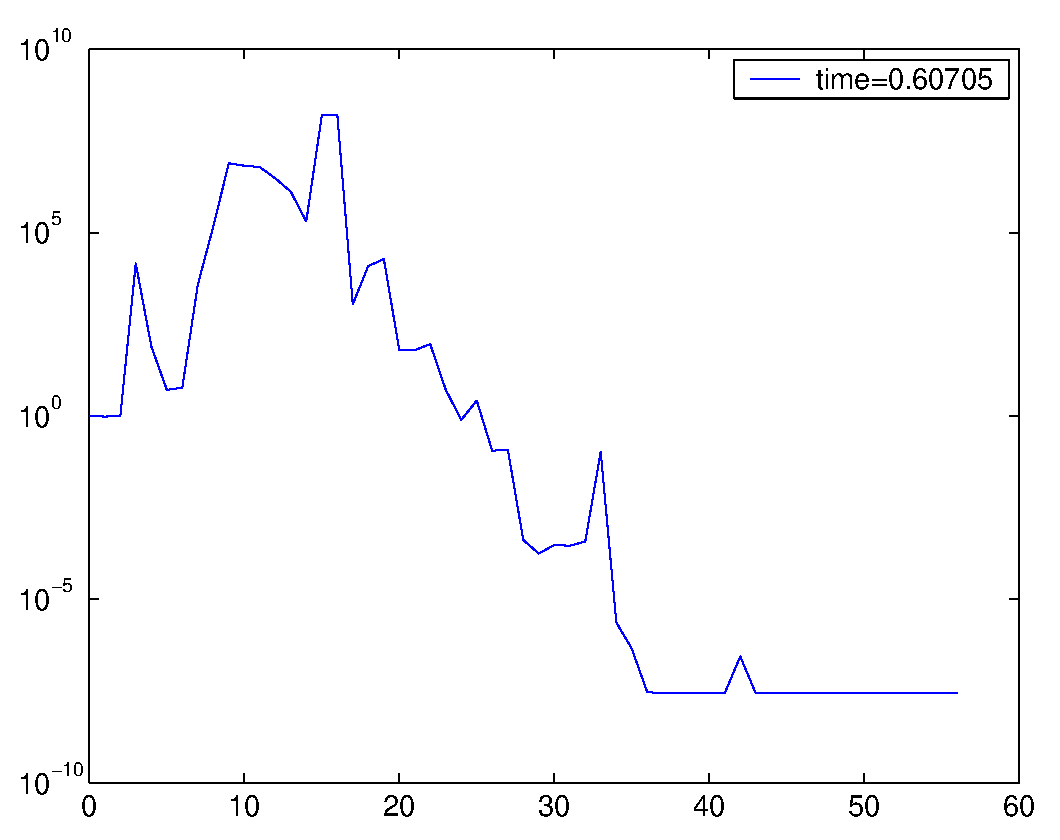
\includegraphics[scale=0.35]{eps/mp3cgsN20e50.eps}\hfill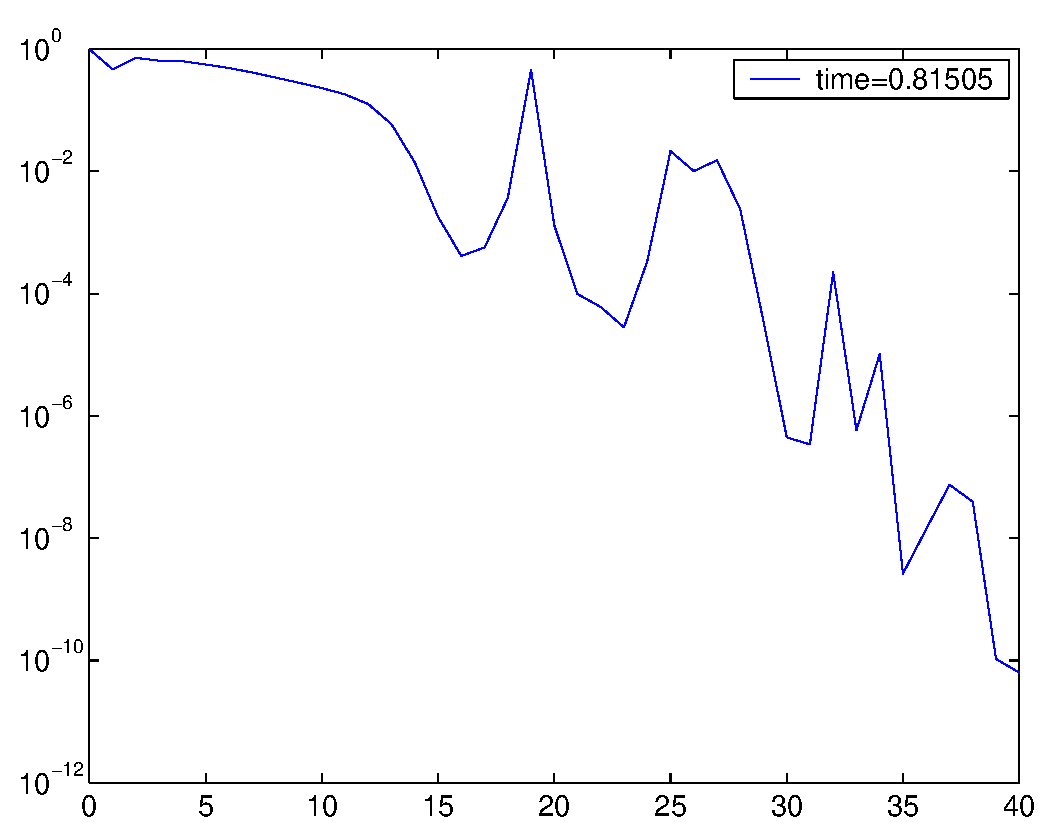
\includegraphics[scale=0.35]{eps/mp3cgsN20e1.eps}
\caption{Konvergenzgeschichte f"ur CGS, Modellproblem III. Links:$N=20,
\epsilon = 50$, rechts $N=20, \epsilon = 1$. Man beachte f"ur 
$\epsilon = 50$ die Stagnation bei $10^{-8}$.}
\end{figure}


\textbf{Neue Idee:} \\Nehme $\Phi_k = \chi_k \varphi_k$ und $\Psi_k = \chi_k \psi_k$, wobei $\chi_k(t)= \prod^{k-1}_{i=1}\left(1-\dfrac{t}{\omega_i}\right)$, $\omega_i$
geeignet gew\"ahlt zur Stabilisierung des Verfahrens. Dann gilt
\begin{align*}
\Phi_{k+1} &= \chi_{k+1}\varphi_{k+1}\\
&= \prod_{i=0}^k \left( 1 - \dfrac{t}{\omega_i} \right) \varphi_{k+1} \\
&= \prod_{i=0}^k \left( 1 - \dfrac{t}{\omega_i} \right) \left( \varphi_k - \gamma_k \vartheta\psi_k \right) \\
&= \left( 1 - \dfrac{t}{\omega_k} \right) \chi_k\left( \varphi_k - \gamma_k \vartheta\psi_k \right)\\
&= \left( 1 - \dfrac{t}{\omega_k} \right)\left( \Phi_k - \gamma_k \vartheta \Psi_k \right)
\end{align*}
sowie
\begin{align*}
 \Psi_{k+1} &= \chi_{k+1}\psi_{k+1}\\
&= \left( 1 - \dfrac{t}{\omega_k} \right) \chi_k\left( \varphi_{k+1} + \rho_k \psi_k \right)\\
&= \Phi_{k+1} + \rho_k \left( 1 - \dfrac{t}{\omega_k} \right) \Psi_k.
\end{align*}

\textbf{Fragen:}
\begin{enumerate}
\item Wie f\"uhrt man eine geeignete Wahl von $\omega_k$ durch ?
\item Wie bekommt man die alten BiCG Koeffizienten $\gamma_k$ und $\rho_k$ aus den neuen Verfahrenspolynomen zur\"uckgewonnen ?
\end{enumerate}

Wir versuchen zuerst, die alten BiCG-Koeffizienten aus den neuen Verfahrenspolynomen zur\"uckzugewinnen.

\begin{lem}
Es gilt:
\begin{enumerate}
\item $ \left[ \varphi_k, p_{k-1} \right] = 0 \quad \forall p_{k-1} \in \Pi_{k-1}$
\item $ \left[ \psi_k, \vartheta p_{k-1} \right] = 0 \quad \forall p_{k-1} \in \Pi_{k-1} $
\end{enumerate}
\end{lem}
\begin{proof}
\begin{enumerate}
\item Nach Konstruktion des BiCG erf\"ullt (Petrov-Galerkin-Bedingung).
\item Beweis per Induktion:
\[
\left[ \psi_k, \vartheta p_{k-2} \right] = 0 \quad \text{nach Induktion und Teil 1}
\]
\[
\left[\psi_k, \vartheta \varphi_{k-1} \right] = \left[ \vartheta \psi_k , \varphi_{k-1} \right] = \left[ \dfrac{\left[ \psi_k , \vartheta \psi_k \right]}{\left[\varphi_k, \varphi_k \right]} \left(\varphi_k - \varphi_{k+1} \right), \varphi_{k-1} \right] = 0.
\]
\end{enumerate}
\end{proof}

\textbf{Folgerung:}
\[
\left[\varphi_k, \varphi_k \right] = \left[ \prod_{i=0}^{k-1} ( - \gamma_i) \vartheta^k + p_{k-1}, \varphi_k \right] = \left[ \prod_{i=0}^{k-1} ( - \gamma_i) \vartheta^k , \varphi_k \right] =\prod_{i=0}^{k-1} ( - \gamma_i) \left[  \vartheta^k , \varphi_k \right].
\]
Also gilt:
\[
\left[ \Phi_k,1 \right] = \left[ \prod_{i=0}^{k-1} \left(1 - \dfrac{t}{\omega_i} \right), \varphi_k \right] = \prod_{i=0}^{k-1} \left(-\dfrac{1}{\omega_i} \right) \left[ \vartheta^k,\varphi_k \right].
\]
Ebenso rechnet man nach, dass gilt:
\[
\left[ \psi_k, \vartheta \psi_k \right] = \left[ \vartheta \psi_k, \psi_k \right] = \left[ \vartheta \psi_k, \prod_{i=0}^{k-1} \left( - \gamma_i \right) \vartheta^k \right] =\prod_{i=0}^{k-1} \left( - \gamma_i \right) \left[ \vartheta \psi_k,  \vartheta^k \right],
\]
\[
\left[ \Psi_k, \vartheta \right] = \left[ \vartheta \Psi_k,1 \right] = \left[ \vartheta \psi_k, \prod_{i=0}^{k-1} \left( 1 - \dfrac{t}{\omega_i} \right) \right] = \prod_{i=0}^{k-1} \left( - \dfrac{1}{\omega_i} \right) \left[ \vartheta \psi_k,\vartheta^k  \right].
\]
Daraus leitet sich folgender Zusammenhang her:
\[
\left[ \varphi_k, \varphi_k \right] = \left[ \Phi_k, 1 \right]  \prod_{i=0}^{k-1} \left( \gamma_i \omega_i \right)
\]
\[
\left[ \psi_k, \vartheta \psi_k \right] = \left[ \Psi_k, \vartheta \right] \prod_{i=0}^{k-1} \left( \gamma_i \omega_i \right)
\]
und damit
\[
\gamma_k = \dfrac{\left[ \varphi_k, \varphi_k \right] }{ \left[ \psi_k, \vartheta \psi_k \right] } = \dfrac{\left[ \Phi_k,1 \right]}{\left[ \Psi_k, \vartheta \right] },
\]
\[
\rho_k = \dfrac{\left[ \varphi_{k+1}, \varphi_{k+1} \right]}{\left[ \varphi_k, \varphi_k \right] } = \gamma_k \omega_k \dfrac{\left[ \Phi_{k+1},1 \right] }{ \left[  \Phi_k, 1 \right] }.
\]

Jetzt bleibt noch, eine passende Wahl der $\omega_k$ zu finden.
Setze \[s^k = \Phi_k(A)r^0 - \gamma_k \vartheta \Psi_k(A) r^0,\] dann ist $s^k$ ein Residuum zu einer Zwischen\-ite\-rier\-ten $y^k$, denn
$\Phi_k(0) - \gamma_k \Psi_k(0) =1$.
W\"ahle $\omega_k$ so das $\| \left( 1 - \dfrac{1}{\omega_k}A \right) s^k \|_2$ minimal wird, was nach Lemma~\ref{minimierungs_lem} f\"ur
\[
\omega_k = \dfrac{\langle As^k, As^k \rangle}{\langle s^k, A s^k \rangle}
\]
der Fall ist. Damit ergibt sich folgender BiCG-Stab Algorithmus:

\begin{alg}[BiCG-Stab, van der Vorst, 1992]
~               % um "Algorithmus" aus dem Kasten rauszubekommen
\vspace*{-2\baselineskip}       % um den Leeraum zu entfernen
\begin{algorithm}
  \begin{algorithmic}
    \STATE w\"ahle $x^0$, setze $r^0 = b-Ax^0$, $p^0 = r^0$, w"ahle $\tilde{r}^0$
    \FOR{$k = 0,1, \dots$ }
      	\STATE $u^k = A p^k$
	\STATE $\gamma_k = \dfrac{\langle r^k, \tilde{r}^0 \rangle}{\langle u^k, \tilde{r}^0 \rangle} $
	\STATE $s^k = r^k - \gamma_k u^k$
	\STATE $v^k = A s^k$
	\STATE $\omega_k = \dfrac{\langle v^k, v^k \rangle}{\langle s^k, v^k \rangle} $
	\STATE $r^{k+1}=s^k - \dfrac{1}{\omega_k} v^k$
	\STATE $\rho_k = \gamma_k \omega_k \dfrac{\langle r^{k+1}, \tilde{r}^0 \rangle}{\langle r^k, \tilde{r}^0 \rangle}$
	\STATE $p^{k+1} = r^{k+1} + \rho_k p_k - \dfrac{\rho_k}{\omega_k} u^k$
	\STATE $x^{k+1} = x^k + \dfrac{1}{\omega_k} s^k + \gamma_k p^k$
    \ENDFOR
  \end{algorithmic}
\end{algorithm}
\end{alg}

\begin{aufg}
Wende BiCG-Stab auf das Modellproblem III an.
\end{aufg}
\begin{figure}[h!]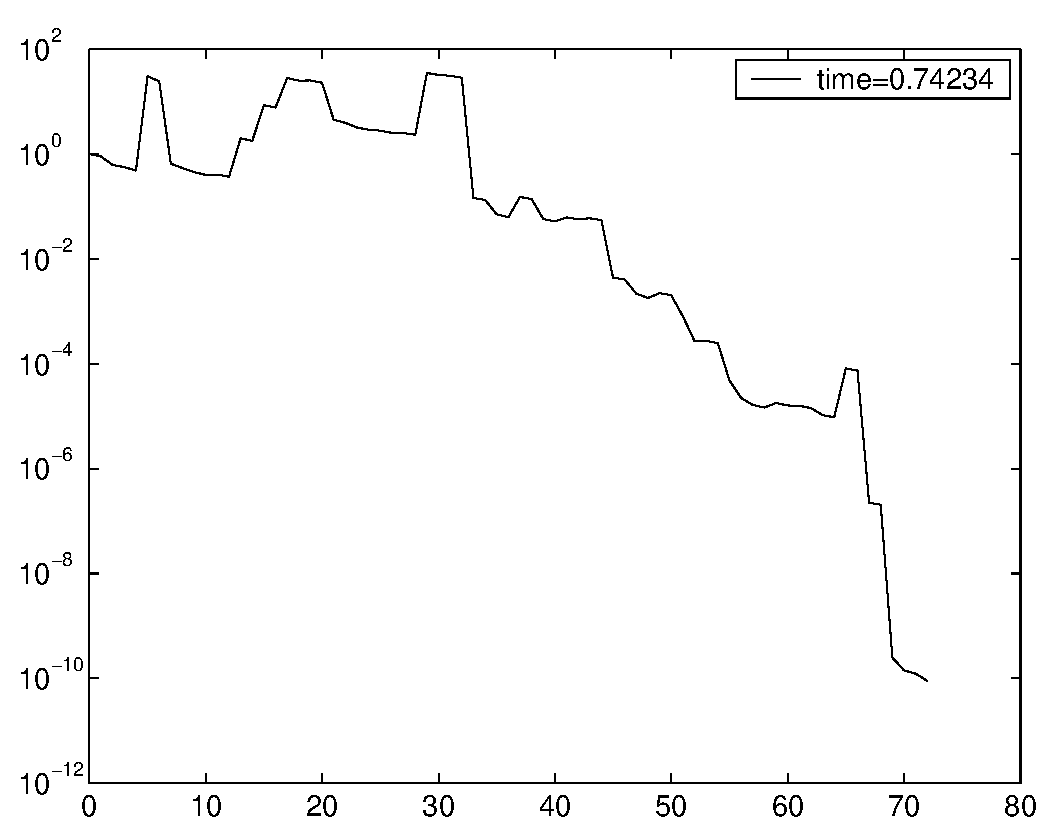
\includegraphics[scale=0.35]{eps/bicgstabN20-e50.eps}\hfill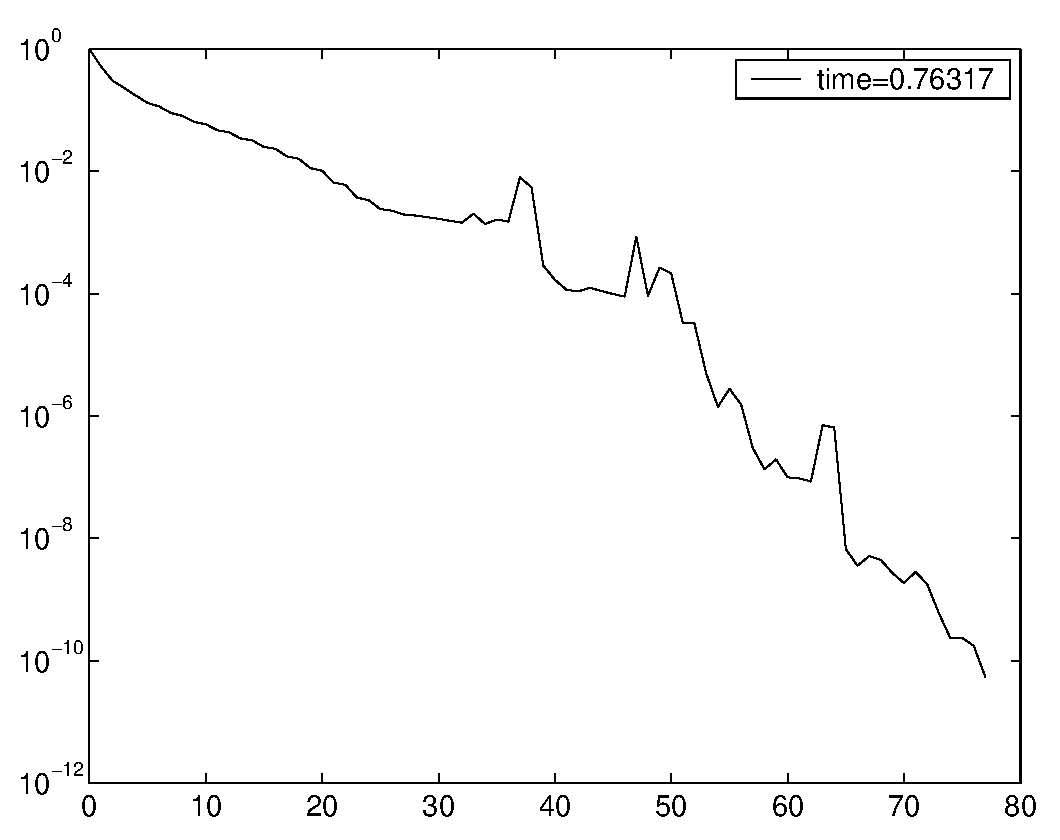
\includegraphics[scale=0.35]{eps/bicgstabN20-e1.eps}\caption{Konvergenzgeschichte f"ur BiCGStab, Modellproblem III. Links:$N=20, \epsilon = 50$, rechts $N=20, \epsilon = 1$. Man beachte die Verbesserungen gegen"uber CGS.}\end{figure}
\begin{bem}
BiCG-Stab ist sehr beliebt, da 2 MVM mit $A$ pro Schritt n\"otig sind und $r^k \in K_{2k}(A,r^0)$. Au\ss erdem ist die Konvergenz relativ glatt.
\end{bem}

